\documentclass[xelatex,aspectratio=169]{beamer}

\hfuzz=10pt
\vfuzz=10pt

% Theme
\usetheme{htw}
\setbeamertemplate{navigation symbols}{}
\setbeamertemplate{theorems}[numbered]
\setbeamercovered{transparent}

%\logo{
\includegraphics[height=0.5cm]{HTWD_color.png}}

% Packages
\usepackage{polyglossia}
\setmainlanguage{german}
\setotherlanguage{english}

\usepackage[bigfiles]{pdfbase}
\ExplSyntaxOn
\NewDocumentCommand\embedvideo{smm}{
\group_begin:
\leavevmode
\tl_if_exist:cTF{file_\file_mdfive_hash:n{#3}}{
  \tl_set_eq:Nc\video{file_\file_mdfive_hash:n{#3}}
}{
  \IfFileExists{#3}{}{\GenericError{}{File~`#3'~not~found}{}{}}
  \pbs_pdfobj:nnn{}{fstream}{{}{#3}}
  \pbs_pdfobj:nnn{}{dict}{
    /Type/Filespec/F~(#3)/UF~(#3)
    /EF~<</F~\pbs_pdflastobj:>>
  }
  \tl_set:Nx\video{\pbs_pdflastobj:}
  \tl_gset_eq:cN{file_\file_mdfive_hash:n{#3}}\video
}
%
\pbs_pdfobj:nnn{}{dict}{
  /Type/RichMediaInstance/Subtype/Video
  /Asset~\video
  /Params~<</FlashVars (
  source=#3&
  skin=SkinOverAllNoFullNoCaption.swf&
  skinAutoHide=true&
  skinBackgroundColor=0x5F5F5F&
  skinBackgroundAlpha=0.75
  )>>
}
%
\pbs_pdfobj:nnn{}{dict}{
/Type/RichMediaConfiguration/Subtype/Video
/Instances~[\pbs_pdflastobj:]
}
%
\pbs_pdfobj:nnn{}{dict}{
/Type/RichMediaContent
/Assets~<<
/Names~[(#3)~\video]
>>
/Configurations~[\pbs_pdflastobj:]
}
\tl_set:Nx\rmcontent{\pbs_pdflastobj:}
%
\pbs_pdfobj:nnn{}{dict}{
  /Activation~<<
  /Condition/\IfBooleanTF{#1}{PV}{XA}
  /Presentation~<</Style/Embedded>>
  >>
  /Deactivation~<</Condition/PI>>
}
%
\hbox_set:Nn\l_tmpa_box{#2}
\tl_set:Nx\l_box_wd_tl{\dim_use:N\box_wd:N\l_tmpa_box}
\tl_set:Nx\l_box_ht_tl{\dim_use:N\box_ht:N\l_tmpa_box}
\tl_set:Nx\l_box_dp_tl{\dim_use:N\box_dp:N\l_tmpa_box}
\pbs_pdfxform:nnnnn{1}{1}{}{}{\l_tmpa_box}
%
\pbs_pdfannot:nnnn{\l_box_wd_tl}{\l_box_ht_tl}{\l_box_dp_tl}{
  /Subtype/RichMedia
  /BS~<</W~0/S/S>>
  /Contents~(embedded~video~file:#3)
  /NM~(rma:#3)
  /AP~<</N~\pbs_pdflastxform:>>
  /RichMediaSettings~\pbs_pdflastobj:
  /RichMediaContent~\rmcontent
}
\phantom{#2}
\group_end:
}
\ExplSyntaxOff


\usepackage{graphicx}
\usepackage[export]{adjustbox}
\usepackage{animate}
%\usepackage[dvipdfmx]{movie15_dvipdfmx}
\usepackage{media9}
\usepackage{tabularx}
\usepackage{colortbl}
\usepackage{booktabs}
\usepackage{makecell}
\usepackage{ltablex}
\usepackage{array}
\usepackage{multirow}
\usepackage{amsmath}
\usepackage{amsthm}
%\renewcommand{\arraystretch}{1.5}
\newcolumntype{L}[1]{>{\raggedright\let\newline\\\arraybackslash\hspace{0pt}}p{#1}}
\newcolumntype{C}[1]{>{\centering\let\newline\\\arraybackslash\hspace{0pt}}p{#1}}
\newcolumntype{R}[1]{>{\raggedleft\let\newline\\\arraybackslash\hspace{0pt}}p{#1}}
%\renewcommand\thesatz{\arabic{section}.\arabic{theorem}}
\makeatletter
\@addtoreset{theorem}{lecture}
\makeatother

\newtheorem{satz}{Satz}[section]
\newtheorem{lem}{Lemma}[section]
\newtheorem{beh}{Behauptung}[section]
\newtheorem{define}{Definition}[section]
\numberwithin{equation}{section}
\usepackage{ragged2e}
\usepackage{etoolbox}

\usepackage{color}
\usepackage{colortbl}
\definecolor{hellgrau}{rgb}{0.85,0.85,0.85}
\definecolor{hellrot}{rgb}{1,0.7,0.7}

\usepackage{tikz}
\usetikzlibrary{shapes,arrows.meta,calc,arrows,positioning,patterns,tikzmark}
%\usepackage{tikz-uml}
\usepackage{pgfplots}  % for elliptic curves (part 8)
\pgfplotsset{compat=1.18}
\usepackage{pgffor}
\usepackage{pgfmath-xfp}
\tikzset{>=latex}
\tikzset{
  invisible/.style={opacity=0},
  visible on/.style={alt={#1{}{invisible}}},
  alt/.code args={<#1>#2#3}{%
      \alt<#1>{\pgfkeysalso{#2}}{\pgfkeysalso{#3}} % \pgfkeysalso doesn't change the path
    },
}

\usepackage{paralist}

\usepackage{url}
\def\UrlBreaks{\do\/\do-}
\PassOptionsToPackage{hyphens}{url}\usepackage{hyperref}

\usepackage[normalem]{ulem} % gestrichelte Unterstreichung (\dashuline{})
\usepackage{cancel}

\makeatletter
\renewcommand{\itemize}[1][]{%
  \beamer@ifempty{#1}{}{\def\beamer@defaultospec{#1}}%
  \ifnum \@itemdepth >2\relax\@toodeep\else
    \advance\@itemdepth\@ne
    \beamer@computepref\@itemdepth% sets \beameritemnestingprefix
    \usebeamerfont{itemize/enumerate \beameritemnestingprefix body}%
    \usebeamercolor[fg]{itemize/enumerate \beameritemnestingprefix body}%
    \usebeamertemplate{itemize/enumerate \beameritemnestingprefix body begin}%
    \list
    {\usebeamertemplate{itemize \beameritemnestingprefix item}}
    {\def\makelabel##1{%
        {%
            \hss\llap{{%
                  \usebeamerfont*{itemize \beameritemnestingprefix item}%
                  \usebeamercolor[fg]{itemize \beameritemnestingprefix item}##1}}%
          }%
      }%
    }
  \fi%
  \beamer@cramped%
  \justifying% NEW
  %\raggedright% ORIGINAL
  \beamer@firstlineitemizeunskip%
}
\makeatother

\apptocmd{\frame}{}{\justifying}{}

\renewcommand\theadfont{\bfseries\sffamily}
\usepackage{ragged2e}
\usepackage{newpxtext}

\setsansfont{texgyreheros}[
  Scale=MatchLowercase,
  UprightFont=*-regular,
  BoldFont=*-bold,
  ItalicFont=*-italic,
  BoldItalicFont=*-bolditalic,
]

% Title
\usepackage[usetransparent=false]{svg}
% Import references
\usepackage[backend=biber,style=numeric,sorting=none]{biblatex}
\addbibresource{references.bib}

%\AtBeginSection[]{
%  \begin{frame}
%    \vfill
%    \centering
%    \begin{beamercolorbox}[sep=8pt,center,shadow=true,rounded=true]{title}
%      \usebeamerfont{title}\thesection.~\secname\par%
%    \end{beamercolorbox}
%    \vfill
%  \end{frame}
%}

\makeatletter
\newenvironment{noheadline}{
  \setbeamertemplate{headline}{}
  \addtobeamertemplate{frametitle}{\vspace*{-0.9\baselineskip}}{}
}{}
\makeatother


\usepackage{xcolor}
\usepackage{algorithm}
\usepackage[linesnumbered,ruled,lined,commentsnumbered,algo2e,ngerman,ngermankw]{algorithm2e}
\usepackage{algorithmic}
\usepackage{caption}
\usepackage[newfloat]{minted}
\captionsetup[listing]{position=top}
\definecolor{mintedbg}{HTML}{282828}
\setminted{
  breaklines=true,
  bgcolor=mintedbg,
  style=monokai,
  formatcom=\color{white}
}
\usepackage{etoolbox}
\makeatletter
% replace \medskip before and after the box with nothing, i.e., remove it
\patchcmd{\minted@colorbg}{\medskip}{}{}{}
\patchcmd{\endminted@colorbg}{\medskip}{}{}{}
\makeatother

\renewcommand{\theFancyVerbLine}{\textcolor{black}{\arabic{FancyVerbLine}}}

\usepackage{pifont}
\newcommand{\cmark}{\ding{51}}%
\newcommand{\xmark}{\ding{55}}%

\newenvironment{changemargin}[2]{%
  \begin{list}{}{%
      \setlength{\topsep}{0pt}%
      \setlength{\leftmargin}{#1}%
      \setlength{\rightmargin}{#2}%
      \setlength{\listparindent}{\parindent}%
      \setlength{\itemindent}{\parindent}%
      \setlength{\parsep}{\parskip}%
    }%
    \item[]}{\end{list}}


\usepackage{csquotes}

% Title
\title{Codierung von Zeichen und Zeichenketten}
\author{Prof. Dr. Lukas Iffländer}
\institute{HTW Dresden}
\date{}
\usepackage{svg}

% Begin document
\begin{document}

% Title slide
\begin{frame}
    \titlepage
\end{frame}

% Section: Motivation/Beispiele
\section{Motivation/Beispiele}

\begin{frame}{Motivation – Interpretation einer Bitfolge}
    \begin{center}
        \begin{tabular}{lccccc}
            \toprule
            Bits      & 01001100 & 01110101 & 01101011 & 01100001 & 01110011 \\
            \midrule
            Hex       & 4C       & 75       & 6B       & 61       & 73       \\
            \midrule
            Buchstabe & L        & u        & k        & a        & s        \\
            \bottomrule
        \end{tabular}
    \end{center}
    \begin{alertblock}{Frage:}
        Woher wissen wir, welcher Buchstabe hinter welchem Code steckt?
    \end{alertblock}
\end{frame}

\begin{frame}{Motivation 1: Internationalized Domain Name (IDN)}
    \begin{alertblock}{Problem}
        \begin{itemize}
            \item Homographischer Angriff: kyrillisches \textit{a} vs. lateinisches
            \item Beispiel: Domain sieht aus wie "apple"
        \end{itemize}

    \end{alertblock}
    \begin{columns}
        \begin{column}{0.5\textwidth}
            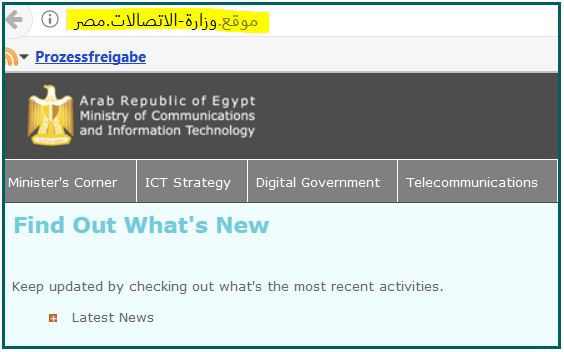
\includegraphics[width=\textwidth]{img/codierung_arabic.png}
        \end{column}
        \begin{column}{0.5\textwidth}
            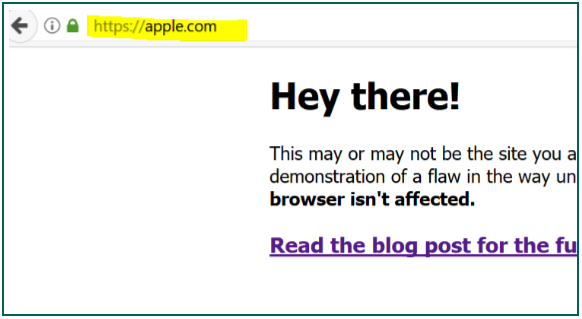
\includegraphics[width=\textwidth]{img/codierung_cyrillic_a.png}
        \end{column}
    \end{columns}
\end{frame}

\begin{frame}{Motivation 2: Numerische Zeichenreferenzen}
    \begin{alertblock}{\enquote{Problem}}
        \begin{itemize}
            \item HTML NCR: \&\#x5350; verweist auf Unicode-Codepoint
            \item Beispiel Swastika auf Google Trends
        \end{itemize}

    \end{alertblock}
    \begin{columns}
        \begin{column}{0.5\textwidth}
            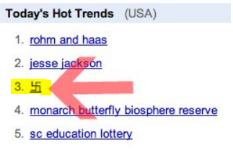
\includegraphics[width=\textwidth]{img/codierung_swastika_1.png}
        \end{column}
        \begin{column}{0.5\textwidth}
            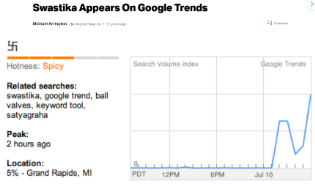
\includegraphics[width=\textwidth]{img/codierung_swastika_2.png}
        \end{column}
    \end{columns}
\end{frame}

\begin{frame}{Motivation 3: Sonderzeichen/Umlaute}
    \begin{block}{Anforderung}
        Wir wollen verschiedene Sprachen unterstützen
    \end{block}
    \begin{alertblock}{Problem}
        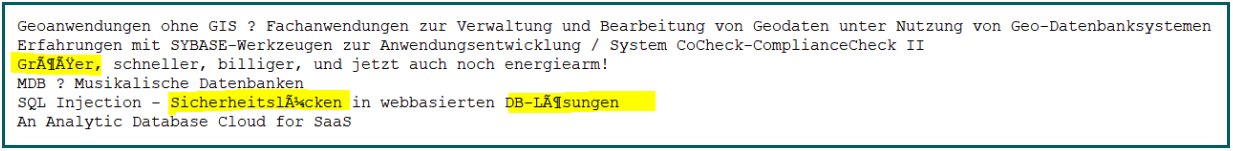
\includegraphics[width=\textwidth]{img/codierung_unicode_fail.png}
    \end{alertblock}
\end{frame}

\begin{frame}{Motivation 4: "Textbomben" / Unicode-Bugs}
    \begin{columns}
        \begin{column}{0.5\textwidth}
            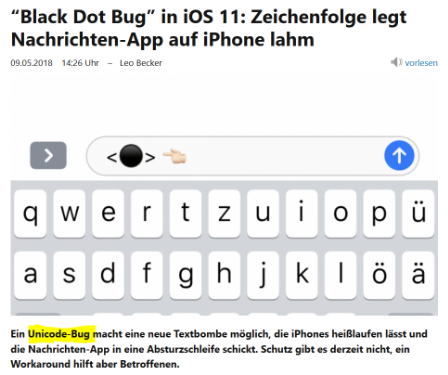
\includegraphics[width=\textwidth]{img/codierung_unicode_bomb_1.png}
        \end{column}
        \begin{column}{0.5\textwidth}
            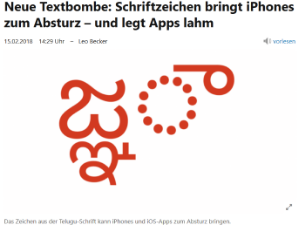
\includegraphics[width=\textwidth]{img/codierung_unicode_bomb_2.png}
        \end{column}
    \end{columns}
\end{frame}

% Section: Terminologie und Geschichte
\section{Terminologie und Geschichte}

\begin{frame}{Zeichenvorrat und Alphabet}
    \begin{block}{Definition: Zeichenvorrat (engl. Character Repertoire, CR)}
        Menge von Zeichen (ungeordnet)
        \begin{itemize}
            \item Menge aller Großbuchstaben (A, B, C, \dots, X, Y, Z)
                  \begin{itemize}
                      \item 26-elementiger Zeichenvorrat
                  \end{itemize}
            \item Menge aller Ziffern (0, 1, 2, \dots, 9)
                  \begin{itemize}
                      \item 10-elementiger Zeichenvorrat
                  \end{itemize}
            \item Binärer Zeichenvorrat
        \end{itemize}
    \end{block}
    \begin{block}{Definition: Alphabet}
        Geordneter Zeichenvorrat
    \end{block}
    \begin{block}{Definition Wort}
        Ein Wort $w$ der Länge $n$ über einen Zeichenvorrat $A$ ist eine endliche Folge $w = a_1 a_2 \ldots a_n \quad \vert \quad a_i \in A \mbox{ und } i \in \mathbb{N}$
    \end{block}
\end{frame}


\begin{frame}{Kurze Geschichte der Zeichencodierung}
    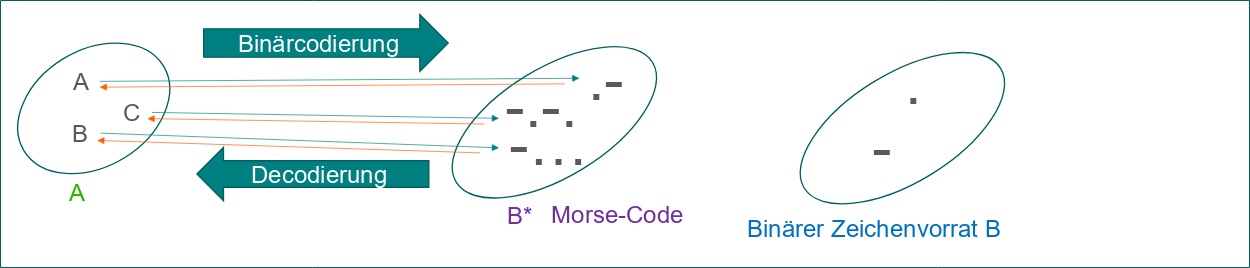
\includegraphics[width=\textwidth]{img/codierung_morsecode.png}
    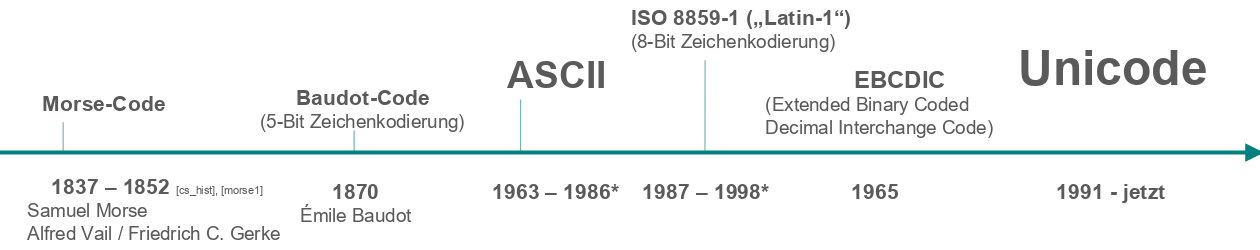
\includegraphics[width=\textwidth]{img/codierung_zeitstrahl.png}
\end{frame}

%\begin{frame}{Terminologie}{Zeichensatz vs. Zeichenkodierung}
%  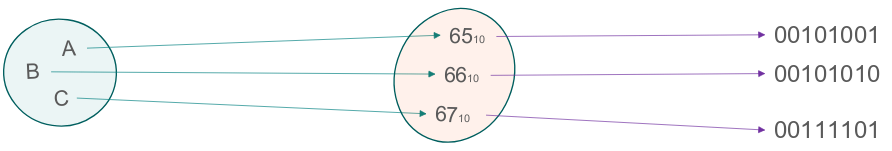
\includegraphics[width=\textwidth]{img/codierung_buchstabe_ccr_byte.png}
%  \begin{tabularx}{\textwidth}{lllX}
%    \toprule
%    Zeichenvorrat          & Zeichenvorrat                & Repräsentation/Bytes        & Definitionsgrundlage            \\
%    (ungeordnet)           & (geordnet)                   &                             &                                 \\
%    \midrule
%    Zeichensatz            & codierter Zeichensatz        & Zeichenkodierung            & World Wide Web Consortium (W3C) \\
%    \textit{Character Set} & \textit{Coded Character Set} & \textit{Character Encoding} &                                 \\
%    \midrule
%  \end{tabularx}
%
%
%\end{frame}

% Section: ASCII
\section{ASCII}


\begin{frame}{ASCII -- American Standard Code for Information Exchange}
    \begin{itemize}
        \item 95 druchbare Zeichen
        \item \textit{33 nicht druckbare Zeichen}
    \end{itemize}

    \begin{exampleblock}{ASCII-Table}
        \centering
        \setlength{\tabcolsep}{0.3em}
        \begin{tabular}{lcccccccccccccccc}
            \toprule
                        & \textbf{x0}  & \textbf{x1}  & \textbf{x2}  & \textbf{x3}  & \textbf{x4}  & \textbf{x5}  & \textbf{x6}  & \textbf{x7}  & \textbf{x8}  & \textbf{x9}       & \textbf{xA}       & \textbf{xB}  & \textbf{xC}      & \textbf{xD} & \textbf{xE} & \textbf{xF}  \\
            \midrule
            \textbf{0x} & \textit{NUL} & \textit{SOH} & \textit{STX} & \textit{ETX} & \textit{EOT} & \textit{ENQ} & \textit{ACK} & \textit{BEL} & \textit{BS}  & \textbackslash{}t & \textbackslash{}n & \textit{VT}  & \textit{FF}      & \textit{CR} & \textit{SO} & \textit{SI}  \\
            \textbf{1x} & \textit{DLE} & \textit{DC1} & \textit{DC2} & \textit{DC3} & \textit{DC4} & \textit{NAK} & \textit{SYN} & \textit{ETB} & \textit{CAN} & \textit{EM}       & \textit{SUB}      & \textit{ESC} & \textit{FS}      & \textit{GS} & \textit{RS} & \textit{US}  \\
            \textbf{2x} & SP           & !            & "            & \#           & \$           & \%           & \&           & '            & (            & )                 & *                 & +            & ,                & -           & .           & /            \\
            \textbf{3x} & 0            & 1            & 2            & 3            & 4            & 5            & 6            & 7            & 8            & 9                 & :                 & ;            & <                & =           & >           & ?            \\
            \textbf{4x} & @            & A            & B            & C            & D            & E            & F            & G            & H            & I                 & J                 & K            & L                & M           & N           & O            \\
            \textbf{5x} & P            & Q            & R            & S            & T            & U            & V            & W            & X            & Y                 & Z                 & [            & \textbackslash{} & ]           & \^{}        & \_           \\
            \textbf{6x} & `            & a            & b            & c            & d            & e            & f            & g            & h            & i                 & j                 & k            & l                & m           & n           & o            \\
            \textbf{7x} & p            & q            & r            & s            & t            & u            & v            & w            & x            & y                 & z                 & \{           & $a$              & \}          & $\sim$      & \textit{DEL} \\
            \bottomrule
        \end{tabular}
    \end{exampleblock}

\end{frame}

\begin{frame}[allowframebreaks]{ASCII -- American Standard Code for Information Exchange}{Nicht druckbare Buchstaben}
    \begin{description}
        \item[NUL] Null character, used to signify the end of a string.
        \item[SOH] Start of Header, used to indicate the start of a header in data transmission.
        \item[STX] Start of Text, marks the beginning of a text block.
        \item[ETX] End of Text, marks the end of a text block.
        \item[EOT] End of Transmission, used to signal the end of data transmission.
        \item[ENQ] Enquiry, used to request a response from a communication partner.
        \item[ACK] Acknowledge, indicates successful receipt of a message.
        \item[BEL] Bell, triggers an audible or visual signal.
        \item[BS] Backspace, moves the cursor one position backward.
        \item[HT] Horizontal Tab, moves the cursor to the next tab stop.
        \item[LF] Line Feed, moves the cursor to the next line.
        \item[VT] Vertical Tab, moves the cursor down to the next vertical tab stop.
        \item[FF] Form Feed, advances the paper to the top of the next page.
        \item[CR] Carriage Return, moves the cursor to the beginning of the line.
        \item[SO] Shift Out, switches to an alternate character set.
        \item[SI] Shift In, switches back to the standard character set.
        \item[DLE] Data Link Escape, used to indicate special control sequences.
        \item[DC1-DC4] Device Control 1-4, used for device-specific controls.
        \item[NAK] Negative Acknowledge, indicates a failure in data transmission.
        \item[SYN] Synchronous Idle, used to maintain synchronization between devices.
        \item[ETB] End of Transmission Block, indicates the end of a block of data.
        \item[CAN] Cancel, used to cancel the current operation.
        \item[EM] End of Medium, indicates the end of a storage medium.
        \item[SUB] Substitute, used to replace an invalid character.
        \item[ESC] Escape, introduces an escape sequence.
        \item[FS] File Separator, separates files in a data stream.
        \item[GS] Group Separator, separates groups of data.
        \item[RS] Record Separator, separates records in a data stream.
        \item[US] Unit Separator, separates units of data.
        \item[DEL] Delete, used to delete a character.
    \end{description}

\end{frame}

\begin{frame}[allowframebreaks]{ASCII -- American Standard Code for Information Exchange}{Eine nützliche Eigenschaft}
    \begin{columns}
        \begin{column}{0.5\textwidth}
            \begin{tabular}{cccc}
                \toprule
                Zeichen & Dezimal & Hexadezimal & Dual     \\
                \midrule
                A       & 65      & 41          & 01000001 \\
                B       & 66      & 42          & 01000010 \\
                \ldots  & \ldots  & \ldots      & \ldots   \\
                Y       & 89      & 59          & 01011001 \\
                Z       & 90      & 5A          & 01011010 \\
                \ldots  & \ldots  & \ldots      & \ldots   \\
                a       & 97      & 61          & 01100001 \\
                b       & 98      & 62          & 01100010 \\
                \ldots  & \ldots  & \ldots      & \ldots   \\
                y       & 121     & 79          & 01111001 \\
                z       & 122     & 7A          & 01111010 \\
                \bottomrule
            \end{tabular}
        \end{column}
        \begin{column}{0.5\textwidth}
            \begin{block}{Abstand zwischen Groß- und Kleinbuchstaben}
                \begin{itemize}
                    \item $A$ bis $Z$ = 65 bis 90
                    \item $a$ bis $z$ = 97 bis 122
                    \item Abstand = 32
                    \item Durch Addition von 32 kann ein Großbuchstabe in einen Kleinbuchstaben umgewandelt werden und umgekehrt.
                \end{itemize}
            \end{block}
        \end{column}
    \end{columns}
\end{frame}

\section{Unicode}

\begin{frame}{Unicode}{Motivation}
    \centering
    
\includegraphics[height=.8\textheight]{img/codierung_scheisse.png}
\end{frame}

\begin{frame}{Unicode}{Entwicklung}
    \begin{itemize}
        \item Entwicklung durch das Unicode Konsortium
        \item (Codierter) Zeichensatz mit erweiterbarem Zeichenvorrat
              \begin{itemize}
                  \item Unicode 1.0 (1991): ~7000 Zeichen
                  \item Unicode 6.0 (2010): ~109.000 Zeichen
                  \item Unicode 12.0 (2019): ~137.000 Zeichen
                  \item Unicode 15.0 (2022): ~149.000 Zeichen
              \end{itemize}
    \end{itemize}
    \begin{block}{Motto}
        Unicode provides a unique number for every character, \\
        no matter what the platform, \\
        no matter what the program, \\
        no matter what the language.
    \end{block}
\end{frame}

\begin{frame}{Unicode}{Anteil der Zeichenkodierungen für Webseiten}
    \begin{tabular}{lcccccccccc}
        \toprule
        in Prozent          & 2010 & 2011 & 2012 & 2013 & 2014 & 2015 & 2016 & 2017 & 2018 & 2019 \\
        \midrule
        \textbf{UTF-8}      & 50.6 & 59.8 & 68.0 & 74.7 & 78.7 & 82.3 & 86.0 & 88.2 & 90.5 & 92.8 \\
        \textbf{ISO-8859-1} & 28.6 & 22.0 & 17.2 & 13.5 & 10.8 & 9.3  & 6.9  & 5.5  & 4.3  & 3.6  \\
        \textbf{US-ASCII}   & 0.2  & 0.1  & 0.1  & 0.1  & 0.1  & 0.1  & <0.1 & <0.1 & <0.1 & <0.1 \\
        \bottomrule
    \end{tabular}
\end{frame}


\begin{frame}{Unicode}{Verfahren -- Planes I}
    \begin{itemize}
        \item Code Space wird 17 gleich große Ebenen (Planes) unterteilt
        \item Jede Plane hat 65.536 Codepunkte ($2^{16}$)
        \item Mit einer vierstelligen Hexadezimalzahl können alle code points innerhalb einer Plane adressiert werden
    \end{itemize}
    \centering
    \begin{tabular}{lcl}
        \toprule
        Plane & Name                                      & Code Range           \\
        \midrule
        0     & Basic Multilingual Plane (BMP)            & U+0000 -- U+FFFF     \\
        1     & Supplementary Multilingual Plane (SMP)    & U+10000 -- U+1FFFF   \\
        2     & Supplementary Ideographic Plane (SIP)     & U+20000 -- U+2FFFF   \\
        3     & Tertiary Ideographic Plane (TIP)          & U+30000 -- U+3FFFF   \\
        5-13  & Unassigned                                & --                   \\
        14    & Supplementary Special-purpose Plane (SSP) & U+E0000 -- U+EFFFF   \\
        15    & Supplementary Private Use Area-A (PUA-A)  & U+F0000 -- U+FFFFF   \\
        16    & Supplementary Private Use Area-B (PUA-B)  & U+100000 -- U+10FFFF \\
        \bottomrule
    \end{tabular}
\end{frame}
\begin{frame}{Unicode}{Verfahren -- Planes II}
    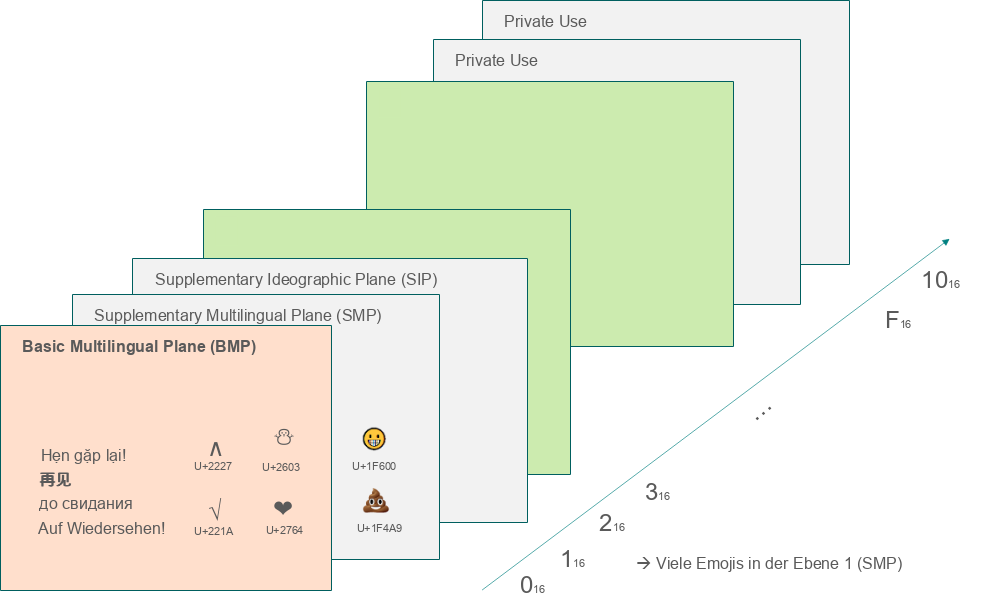
\includegraphics[height=.8\textheight]{img/codierung_planes.png}
\end{frame}

\begin{frame}{Unicode}{Basic Multilingual Plane (BMP)}
    \centering
    \setlength{\tabcolsep}{1em}
    \small
    \begin{tabular}{lcccccccccccccccc}
        \toprule
                        & \textbf{0}                                            & \textbf{1}                         & \textbf{2}                    & \textbf{3}                               & \textbf{4} & \textbf{5} & \textbf{6} & \textbf{7} & \textbf{8} & \textbf{9} & \textbf{A} & \textbf{B} & \textbf{C} & \textbf{D} & \textbf{E} & \textbf{F} \\
        \midrule
        \textbf{00}     & \multicolumn{2}{|c}{C0}                               & \multicolumn{6}{|c}{Basic Latin}   & \multicolumn{2}{|c}{C1}       & \multicolumn{6}{|c|}{Latin 1 Supplement}                                                                                                                                                             \\
        \textbf{01}     &                                                                                                                                                                                                                                                                                                                                   \\
        \textbf{\ldots} &                                                                                                                                                                                                                                                                                                                                   \\
        \textbf{20}     & \multicolumn{7}{|c}{General Punctation}               & \multicolumn{3}{|c}{Subs./Supers.} & \multicolumn{3}{|c}{Currency} & \multicolumn{3}{|c|}{Diac. Symbs.}                                                                                                                                                                   \\
        \textbf{\ldots} &                                                                                                                                                                                                                                                                                                                                   \\
        \textbf{FF}     & \multicolumn{16}{|c| }{Halfwidth and Fullwidth Forms}                                                                                                                                                                                                                                                                             \\
        \bottomrule
    \end{tabular}
\end{frame}

\begin{frame}{Unicode}{Unicode Character Encoding}
    \begin{alertblock}{Frage}
        Wie stellen wir das jetzt im Dualsystem dar?
    \end{alertblock}
    \begin{block}{Begrenzungen}
        \begin{itemize}
            \item Mindestens 17 Planes
            \item Jede Plane hat 65.536 Codepunkte ($2^{16}$)
            \item Wir brauchen also mindestens 17*65.536 = 1.114.112 Codepunkte
            \item Das sind 21 Bit
        \end{itemize}
    \end{block}
\end{frame}

\begin{frame}{Unicode}{The obvious choice: UTF-32}
    \begin{itemize}
        \item UTF-32 ist die einfachste und direkteste Kodierung
        \item Jedes Zeichen wird durch 4 Byte (32 Bit) dargestellt

              32 ist die nächste Potenz von 2, die alle Zeichen abdecken kann
        \item Einfache Implementierung
        \item Hoher Speicherbedarf
        \item Keine Rückwärtskompatibilität zu ASCII
    \end{itemize}
    \begin{block}{Beispiel}
        \begin{itemize}
            \item U+0041 = A = 0x41 = 00000000 00000000 00000000 01000001
            \item U+00C4 = Ä = 0xC4 = 00000000 00000000 00000000 11000100
            \item U+20AC = € = 0x20AC = 00000000 00000000 00100000 10101100
            \item U+1F600 = {\symbolfont 😀} = 0x1F600 = 00000000 00000001 11110110 00000000
        \end{itemize}
    \end{block}
\end{frame}

\begin{frame}{Unicode}{Historisch gewachsen: UTF-16}
    \begin{itemize}
        \item UTF-16 ist eine Kodierung, die 2 oder 4 Byte pro Zeichen verwendet
        \item Die ersten 65.536 Zeichen (BMP) werden mit 2 Byte kodiert wobei 2048 Zeichen
              (U+D800 bis U+DFFF) reserviert sind
        \item Alle anderen Zeichen werden mit 4 Byte kodiert
        \item Dazu werden zwei Codepunkte (Surrogate) aus dem reservierten Bereich
              verwendet
    \end{itemize}
    \begin{block}{Umrechnung Surrogate <-> Codepoint}
        \centering
        \begin{tabular}{lcccc}
            \toprule
            \diagbox{\textbf{High}}{\textbf{Low}} & \textbf{0xDC00} & \textbf{0xDC01} & \textbf{\ldots} & \textbf{0xDFFF} \\
            \midrule
            \textbf{0xD800}                       & 0x010000        & 0x010001        & \ldots          & 0x0103FF        \\
            \textbf{0xD801}                       & 0x010400        & 0x010401        & \ldots          & 0x0107FF        \\
            \textbf{\vdots}                       & $\vdots$        & $\vdots$        & $\ddots$        & $\vdots$        \\
            \textbf{0xDBFF}                       & 0x10FC00        & 0x10FC01        & \ldots          & 0x10FFFF        \\
            \bottomrule
        \end{tabular}

    \end{block}
\end{frame}

\begin{frame}{Unicode}{UTF-16 Encoding}
    \begin{itemize}
        \item Vom Codepoint wird 0x10000 subtrahiert (dadurch passen wir in 20 Bit)
        \item Die ersten 10 Bits werden auf die High Surrogate
              (0xD800) addiert
        \item Die letzten 10 Bits werden auf die Low Surrogate
              (0xDC00) addiert
    \end{itemize}
    \setlength{\tabcolsep}{0.2em}
    \centering
    \small
    \begin{tabular}{lccccccccccccccccccccr}
        \toprule
        Bit: & 00 & 01 & 02 & 03 & 04 & 05 & 06 & 07 & 08 & 09 & 10 & 11 & 12 & 13 & 14 & 15 & 16 & 17 & 18 & 19 &                     \\
        \midrule
        U'   & y  & y  & y  & y  & y  & y  & y  & y  & y  & y  & x  & x  & x  & x  & x  & x  & x  & x  & x  & x  & U - 0x10000         \\
        W1   & 1  & 1  & 0  & 1  & 1  & 0  & y  & y  & y  & y  & y  & y  & y  & y  & y  & y  &    &    &    &    & 0xD800 + yyyyyyyyyy \\
        W2   & 1  & 1  & 0  & 1  & 1  & 1  & x  & x  & x  & x  & x  & x  & x  & x  & x  & x  &    &    &    &    & 0xDC00 + xxxxxxxxxx \\
        \bottomrule
    \end{tabular}

    \begin{exampleblock}{Beispiel {\symbolfont 🚀} (Rakete, Codepunkt U+1F680}

        \centering
        \small
        \begin{tabular}{lccccccccccccccccccccr}
            \toprule
            Bit: & 00 & 01 & 02 & 03 & 04 & 05 & 06 & 07 & 08 & 09 & 10 & 11 & 12 & 13 & 14 & 15 & 16 & 17 & 18 & 19 &                     \\
            \midrule
            U'   & 0  & 0  & 0  & 0  & 1  & 1  & 1  & 1  & 0  & 1  & 1  & 0  & 1  & 0  & 0  & 0  & 0  & 0  & 0  & 0  & U - 0x10000         \\
            W1   & 1  & 1  & 0  & 1  & 1  & 0  & 0  & 0  & 1  & 1  & 1  & 1  & 0  & 1  & 1  & 0  &    &    &    &    & 0xD800 + yyyyyyyyyy \\
            W2   & 1  & 1  & 0  & 1  & 1  & 1  & 1  & 0  & 1  & 0  & 0  & 0  & 0  & 0  & 0  & 0  &    &    &    &    & 0xDC00 + xxxxxxxxxx \\
            \bottomrule
        \end{tabular}
    \end{exampleblock}
\end{frame}

\begin{frame}{Unicode}{UTF-16 Vor- und Nachteile}
    \begin{exampleblock}{Vorteile}
        \begin{itemize}
            \item Effizient für die meistgebrauchten Zeichen (nur 2 Bytes)
            \item Kann alle Unicode-Zeichen darstellen
            \item War historisch wichtig, da 16-Bit-Architekturen verbreitet waren
        \end{itemize}
    \end{exampleblock}
    \begin{alertblock}{Nachteile}
        \begin{itemize}
            \item Variable Länge (1 oder 2 Einheiten pro Zeichen)
            \item Teilweise ineffizient bei nicht-westlichen Schriftsystemen
        \end{itemize}
    \end{alertblock}
\end{frame}

\begin{frame}{Unicode}{The Internet Standard UTF-8}
    \begin{block}{Idee}
        \begin{itemize}
            \item Jeder "unicode scalar value" wird durch 1 bis 4 Bytes dargestellt
            \item ASCII-Zeichen (U+0000 bis U+007F) werden mit 1 Byte kodiert
            \item Alle anderen Zeichen werden mit 2, 3 oder 4 Bytes kodiert
        \end{itemize}
    \end{block}

\end{frame}

\begin{frame}{Unicode}{UTF-8 -- Abbildung}
    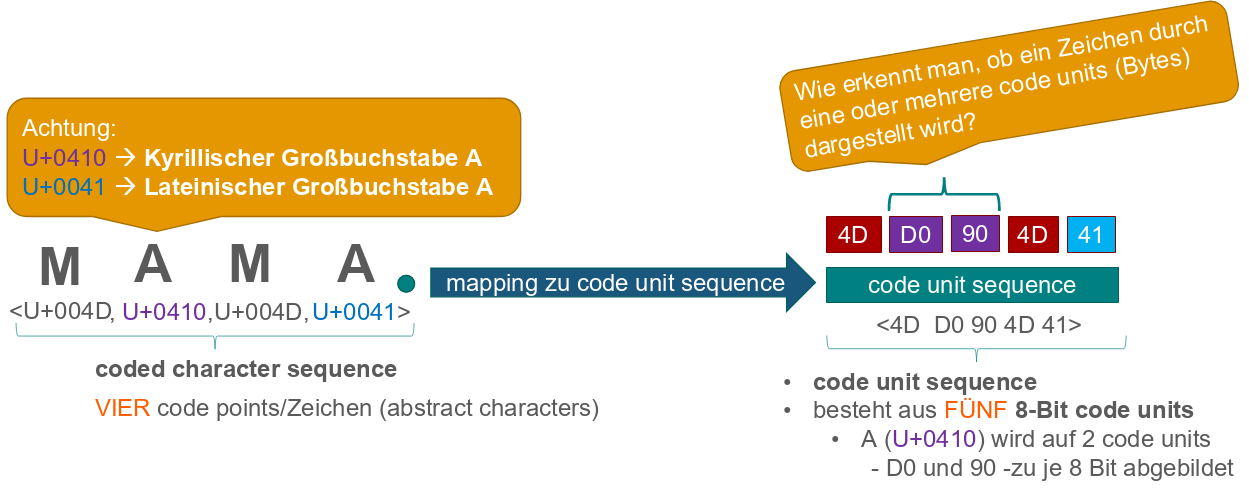
\includegraphics[width=\textwidth]{img/codierung_utf8_abbildung.png}
\end{frame}

\begin{frame}{Unicode}{UTF-8 -- Kodierung}
    \begin{center}
        \begin{tabular}{lr}
            \toprule
            \textbf{Codepoint}           & \textbf{UTF-8}                               \\
            \midrule
            \texttt{U+~0000 -- U+~~007F} & \texttt{0xxxxxxx}                            \\
            \texttt{U+~0080 -- U+~~07FF} & \texttt{110xxxxx 10xxxxxx}                   \\
            \texttt{U+~0800 -- U+~~FFFF} & \texttt{1110xxxx 10xxxxxx 10xxxxxx}          \\
            \texttt{U+10000 -- U+10FFFF} & \texttt{11110xxx 10xxxxxx 10xxxxxx 10xxxxxx} \\
            \bottomrule
        \end{tabular}
    \end{center}
    \begin{block}{Regel}
        \begin{itemize}
            \item Die Anzahl der führenden Einsen gefolgt von einer Null gibt die Anzahl der Bytes an.
            \item Folgebytes beginnen immer mit 10.
            \item Die restlichen Bits sind die Bits des Codepoints.
        \end{itemize}

    \end{block}
\end{frame}
\begin{frame}{Unicode}{UTF-8 -- Kodierung Beispiel}
    \begin{exampleblock}{Beispiel {\symbolfont 💩} (Pile of Poo)}
        \begin{itemize}
            \item U+1F4A9 = 0001 1111 0100 1010 1001
            \item UTF-8: 11110xxx 10xxxxxx 10xxxxxx 10xxxxxx
            \item UTF-8: 11110000 10011111 10011000 10101001
            \item UTF-8: F0 9F 92 A9
        \end{itemize}
    \end{exampleblock}
\end{frame}

\section{Endianness}
\begin{frame}{Endianness}
    \begin{alertblock}{Problem}
        \begin{itemize}
            \item Bytereihenfolge (endianness) ist die Reihenfolge, in der Bytes in einem Wort gespeichert werden.
            \item Abhängig von der Architektur kann die Reihenfolge unterschiedlich sein.
        \end{itemize}
    \end{alertblock}
    \begin{block}{Arten}
        \begin{itemize}
            \item \textbf{Big Endian}: \textbf{M}ost \textbf{S}ignificant \textbf{B}it (MSB) wird zuerst gespeichert.
            \item \textbf{Little Endian}: \textbf{L}east \textbf{S}ignificant \textbf{B}it (LSB) wird zuerst gespeichert.
        \end{itemize}
    \end{block}
    \begin{exampleblock}{Analogie}
        Wir kennen das Phänomen von der Sprache:
        \begin{itemize}
            \item 25 = twenty-five (English, Big Endian)
            \item 25 = fünfundzwanzig (German, Little Endian)
        \end{itemize}
    \end{exampleblock}
\end{frame}

\begin{frame}{Endianness}{Beispiele}
    \begin{columns}
        \begin{column}{0.5\textwidth}
            \begin{exampleblock}{Big Endian}
                \centering
                \begin{tabular}{cccc}
                    \multicolumn{2}{l}{\textcolor{blue}{MSB}} & \multicolumn{2}{r}{\textcolor{olive}{LSB}}                                           \\
                    \toprule
                    \multicolumn{2}{c}{\textbf{Byte 0}}       & \multicolumn{2}{c}{\textbf{Byte 1}}                                                  \\
                    \midrule
                    \textcolor{blue}{\textbf{1}}000           & 1100                                       & 1010 & 000\textcolor{olive}{\textbf{0}} \\
                    0x8                                       & 0xC                                        & 0xA  & 0x0                              \\
                    \bottomrule
                \end{tabular}

            \end{exampleblock}
        \end{column}
        \begin{column}{0.5\textwidth}
            \begin{exampleblock}{Little Endian}
                \centering
                \begin{tabular}{cccc}
                    \multicolumn{2}{r}{\textcolor{olive}{LSB}} & \multicolumn{2}{l}{\textcolor{blue}{MSB}}                                          \\
                    \toprule
                    \multicolumn{2}{c}{\textbf{Byte 0}}        & \multicolumn{2}{c}{\textbf{Byte 1}}                                                \\
                    \midrule
                    1010                                       & 000\textcolor{olive}{\textbf{0}}          & \textcolor{blue}{\textbf{1}}000 & 1100 \\
                    0xA                                        & 0x0                                       & 0x8                             & 0xC  \\
                    \bottomrule
                \end{tabular}
            \end{exampleblock}
        \end{column}
    \end{columns}
\end{frame}

\begin{frame}{Endianness}{Mixed Endianness}
    \begin{alertblock}{Mixed Endianness}
        \begin{itemize}
            \item Mixed Endianness ist eine Kombination aus Big und Little Endian.
            \item Beispiel: 0x12345678 wird als 0x78563412 gespeichert.
        \end{itemize}
    \end{alertblock}
    \begin{exampleblock}{Analogie}
        Wieder Analogie aus der Sprache:
        \begin{itemize}
            \item 125 = hundert fünfundzwanzig (100er zuerst, dann 1er, dann 10er)
        \end{itemize}
    \end{exampleblock}
    \begin{alertblock}{Warnung}
        Mixed Endianness kommt immer, wenn man es nicht erwartet und kann tagelanges Debugging verursachen.
    \end{alertblock}
\end{frame}

\section{Strings in Python}

\begin{frame}{Strings in Python}{Grundlagen}
    \inputminted{python}{src/strings_hello.py}
    \begin{itemize}
        \item Bei einer solchen Zuweisung wird der Datentyp \texttt{str} (kurz für String) verwendet.
        \item Python verwendet derzeit UTF-16 intern (eine Migration auf UTF-8 in \enquote{einer zukünftigen Version} ist geplant).
        \item Einzelnes Zeichen: \mintinline{python}|z = 'x'|
        \item Zeichenkette: \mintinline{python}|s = 'Achtung!'|
        \item Mehrzeilige Strings
              \inputminted{python}{src/strings_multiline.py}
    \end{itemize}
\end{frame}

\begin{frame}{Strings in Python}{Umrechnen in ASCII}
    Funktionen für einzelne Zeichen (Strings der Länge 1):
    \inputminted{python}{src/strings_conversion.py}

\end{frame}

\begin{frame}{Strings in Python}{Ausgewählte Funktionen und Methoden}
    \inputminted{python}{src/strings_functions.py}
\end{frame}

\begin{frame}{Strings in Python}{Vergleichen}
    \inputminted{python}{src/strings_comparison.py}
    \begin{itemize}
        \item Strings können mit den Operatoren \texttt{==}, \texttt{!=}, \texttt{<}, \texttt{<=}, \texttt{>} und \texttt{>=} verglichen werden.
        \item Dabei wird lexikographisch verglichen (wie im Wörterbuch).
        \item Die Vergleiche sind case-sensitive.
    \end{itemize}
\end{frame}

\begin{frame}{Strings in Python}{Teilzeichenketten (Substrings) zählen}
    \inputminted{python}{src/strings_substring_count.py}
    \begin{itemize}
        \item Die Methode \texttt{count()} zählt, wie oft ein Teilstring in einem String vorkommt.
        \item Die Methode ist case-sensitive.
    \end{itemize}
\end{frame}

\begin{frame}{Strings in Python}{Teilzeichenketten (Substrings) finden}
    \inputminted{python}{src/strings_substring_find.py}
    \begin{itemize}
        \item Die Methode \texttt{find()} gibt den Index des ersten Vorkommens eines Teilstrings zurück.
        \item Wenn der Teilstring nicht gefunden wird, gibt die Methode \texttt{-1} zurück.
        \item Die Methode ist case-sensitive.
        \item Die Methode \texttt{rfind()} gibt den Index des letzten Vorkommens eines Teilstrings zurück.
    \end{itemize}
\end{frame}

\begin{frame}{Strings in Python}{Indizierung}
    \inputminted[lastline=3]{python}{src/strings_index.py}
    \begin{itemize}
        \item Strings sind indizierbar und können über Indizes angesprochen werden.
        \item Der Index ist 0-basiert, d.h. der erste Buchstabe hat den Index 0.
        \item Negative Indizes zählen von hinten, d.h. der letzte Buchstabe hat den Index -1.
    \end{itemize}
    \inputminted[firstline=5]{python}{src/strings_index.py}
    \begin{itemize}
        \item Durch die Indizierung mit \texttt{[start:end]} kann ein Teilstring erstellt werden.
        \item Der \texttt{start}-Index ist inklusiv, der \texttt{end}-Index exklusiv (wie bei \texttt{range()}).
        \item Der \texttt{end}-Index kann weggelassen werden, dann wird bis zum Ende des Strings geschnitten.
        \item Der \texttt{start}-Index kann weggelassen werden, dann wird vom Anfang des Strings geschnitten.
    \end{itemize}

\end{frame}

\begin{frame}{Strings in Python}{Indizierung -- Beispiele}
    \inputminted{python}{src/strings_index_examples.py}
\end{frame}

\begin{frame}{Strings in Python}{Zusammensetzung}
    \inputminted{python}{src/strings_concat.py}
    \begin{itemize}
        \item Strings können durch den Operator \texttt{+} zusammengefügt werden.
    \end{itemize}
\end{frame}

\begin{frame}{Strings in Python}{Zusammensetzung längerer Strings -- Alte Methode}
    \begin{columns}
        \begin{column}{0.5\textwidth}
            \begin{itemize}
                \item Programme erfordern das Zusammensetzen von Ausgaben aus numerischen Werten und Strings.
                \item Numerische Werte werden mit \texttt{str()} in Strings umgewandelt und mit \texttt{+} zusammengefügt.
            \end{itemize}
        \end{column}
        \begin{column}{0.5\textwidth}
            \inputminted{python}{src/strings_concat_long_old.py}
        \end{column}
    \end{columns}

\end{frame}

\begin{frame}{Strings in Python}{Zusammensetzung längerer Strings -- Neue Methode}
    \inputminted{python}{src/strings_concat_long_new.py}
    \begin{itemize}
        \item Die neue Methode verwendet f-Strings (ab Python 3.6).
        \item Variablen werden in geschweifte Klammern gesetzt.
        \item Der String wird mit einem \texttt{f} vorangestellt.
    \end{itemize}
\end{frame}

\begin{frame}{Strings in Python}{Ausgabeformatierung mit f-Strings}
    \inputminted{python}{src/strings_concat_long_new_float.py}
    \begin{itemize}
        \item Mit f-Strings können auch Formatierungen vorgenommen werden.
    \end{itemize}
\end{frame}

% End document
\end{document}
